\section{Regression Analysis}
\begin{frame}
\frametitle{Estimation of ET Values}
\tikzproblem{Given a set of features, can we estimate ET?}
\onslide<2->{
\begin{itemize}[<+->]
\setlength\itemsep{1em}
\item Which features to choose?
\item \textit{How well} is our estimate?
\end{itemize}
}
\end{frame}

\begin{frame}
\frametitle{(CIMIS) Penman Monteith Equation for Calculating ET}
\begin{equation*}
\boxed{ET_o = \frac{\bigtriangleup(R_n-G)}{\lambda[\bigtriangleup+\gamma(1+C_du_2)]} + \frac{\gamma\frac{37}{T_a+273.16}u_2(e_s-e_a)}{\bigtriangleup+\gamma(1+C_du_2)}}
\end{equation*}
\onslide<2->{
\tikzstatement{Ultimately depends on four weather features}
\begin{itemize}
\setlength\itemsep{1em}
\item Solar net radiation
\item Vapor pressure
\item Air temperature
\item Wind speed
\end{itemize}
}
\end{frame}

%\begin{frame}
%\frametitle{Scatterplot Matrix of Features of Interest}
%\begin{figure}
%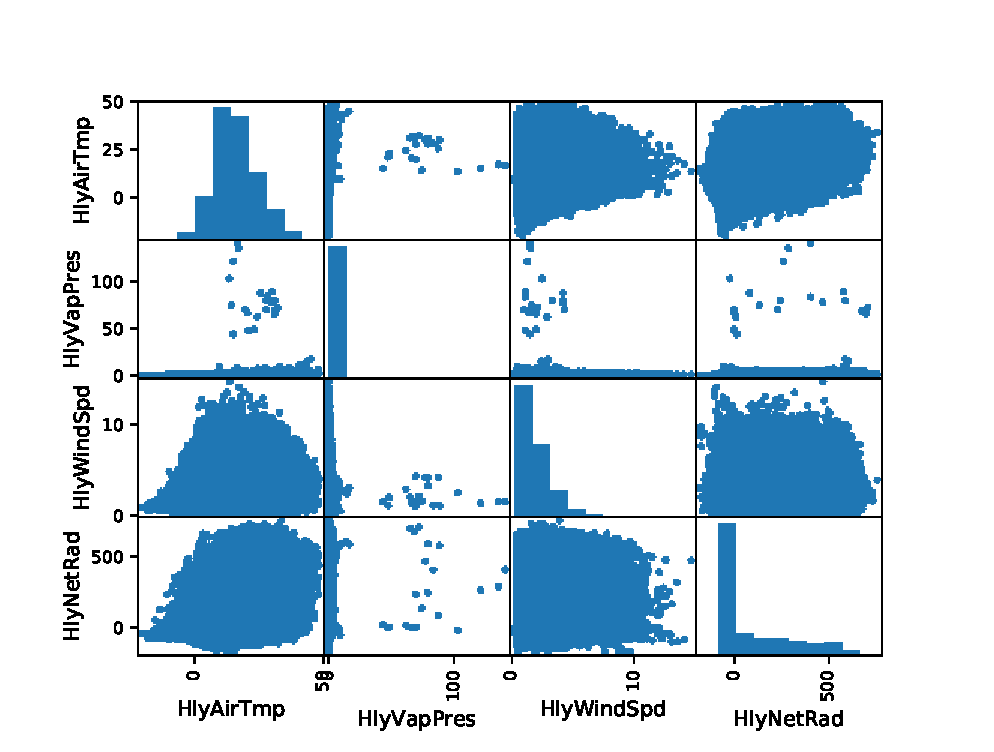
\includegraphics[width=0.85\textwidth]{images/scatterplot-matrix-HlyAirTmp-HlyVapPres-HlyWindSpd-HlyNetRad}
%\end{figure}
%\end{frame}

\begin{frame}
\frametitle{Regression Results}
\footnotesize
\begin{tabular}{|l|l|l|}
\hline
\textbf{Features} & \textbf{Mean Squared Error} & \textbf{$R^2$ Value}\\
\hline
HlyAirTmp,HlyNetRad,HlyVapPres,HlyWindSpd & 0.000970123960314 & 0.981294016164\\
\hline
HlyAirTmp,HlyNetRad,HlyVapPres & 0.00130358866256 & 0.974761220654\\
\hline
HlyAirTmp,HlyNetRad,HlyWindSpd & 0.00131186536214 & 0.974527982555\\
\hline
HlyAirTmp,HlyNetRad & 0.00173654973306 & 0.966537004752\\
\hline
HlyNetRad,HlyVapPres,HlyWindSpd & 0.00248645097725 & 0.952009857384\\
\hline
HlyNetRad,HlyWindSpd & 0.0024909080494 & 0.951659909255\\
\hline
HlyNetRad,HlyVapPres & 0.00302176798112 & 0.941065800356\\
\hline
\only<1>{HlyNetRad}\only<2>{\fcolorbox{red}{white}{HlyNetRad}} & 0.00304665078019 & 0.940955854127\\
\hline
HlyAirTmp,HlyVapPres,HlyWindSpd & 0.0236668111725 & 0.540318481\\
\hline
HlyAirTmp,HlyWindSpd & 0.0242823252297 & 0.528560618195\\
\hline
HlyAirTmp,HlyVapPres & 0.026563048828 & 0.485028160007\\
\hline
HlyAirTmp & 0.0278295291341 & 0.459710153733\\
\hline
HlyVapPres,HlyWindSpd & 0.0407552684279 & 0.208827525819\\
\hline
HlyWindSpd & 0.0412914020576 & 0.196118554063\\
\hline
HlyVapPres & 0.0510006461517 & 0.0128578989128\\
\hline
\end{tabular}
\end{frame}
